%!TEX root = ../report.tex

\begin{document}
    \section{Comparison between GraphQL \& Falcor} \label{sec:graphql_falcor}
	In this section, we are going to analyze the potential features of GraphQL and Falcor, also the possibility of adapting these frameworks as a base for our mediator. Before getting into GraphQL and Falcor, we should know what REST API is and how it transformed the way of communication between systems for many years.
    \subsection{REST API}
	Primarily API stands for Application Programming Interface, and it allows any software to talk with each other. There are different types of API available, but here in the context of GraphQL and Falcor, we consider REST API (REpresentational State Transfer API).  Fundamentally, REST API works in the same way as how websites work. A client sends a request to the server over HTTP protocol, and the client gets an HTML (Hypertext Markup Language) page as a response and browser renders the page. In REST API, the server sends a JSON (Javascript Object Notation) response instead of HTML page. The JSON response might be unreadable to humans, but it is readable by machines. Then the client program parses the response and performs any actions on the data as they wish. 

	This architecture looks perfect for fetching the data from the server but what are the limitations in this architecture that give space for the emergence of frameworks like GraphQL and Falcor?
	
	\begin{figure}[!htbp] 
		\begin{center}
			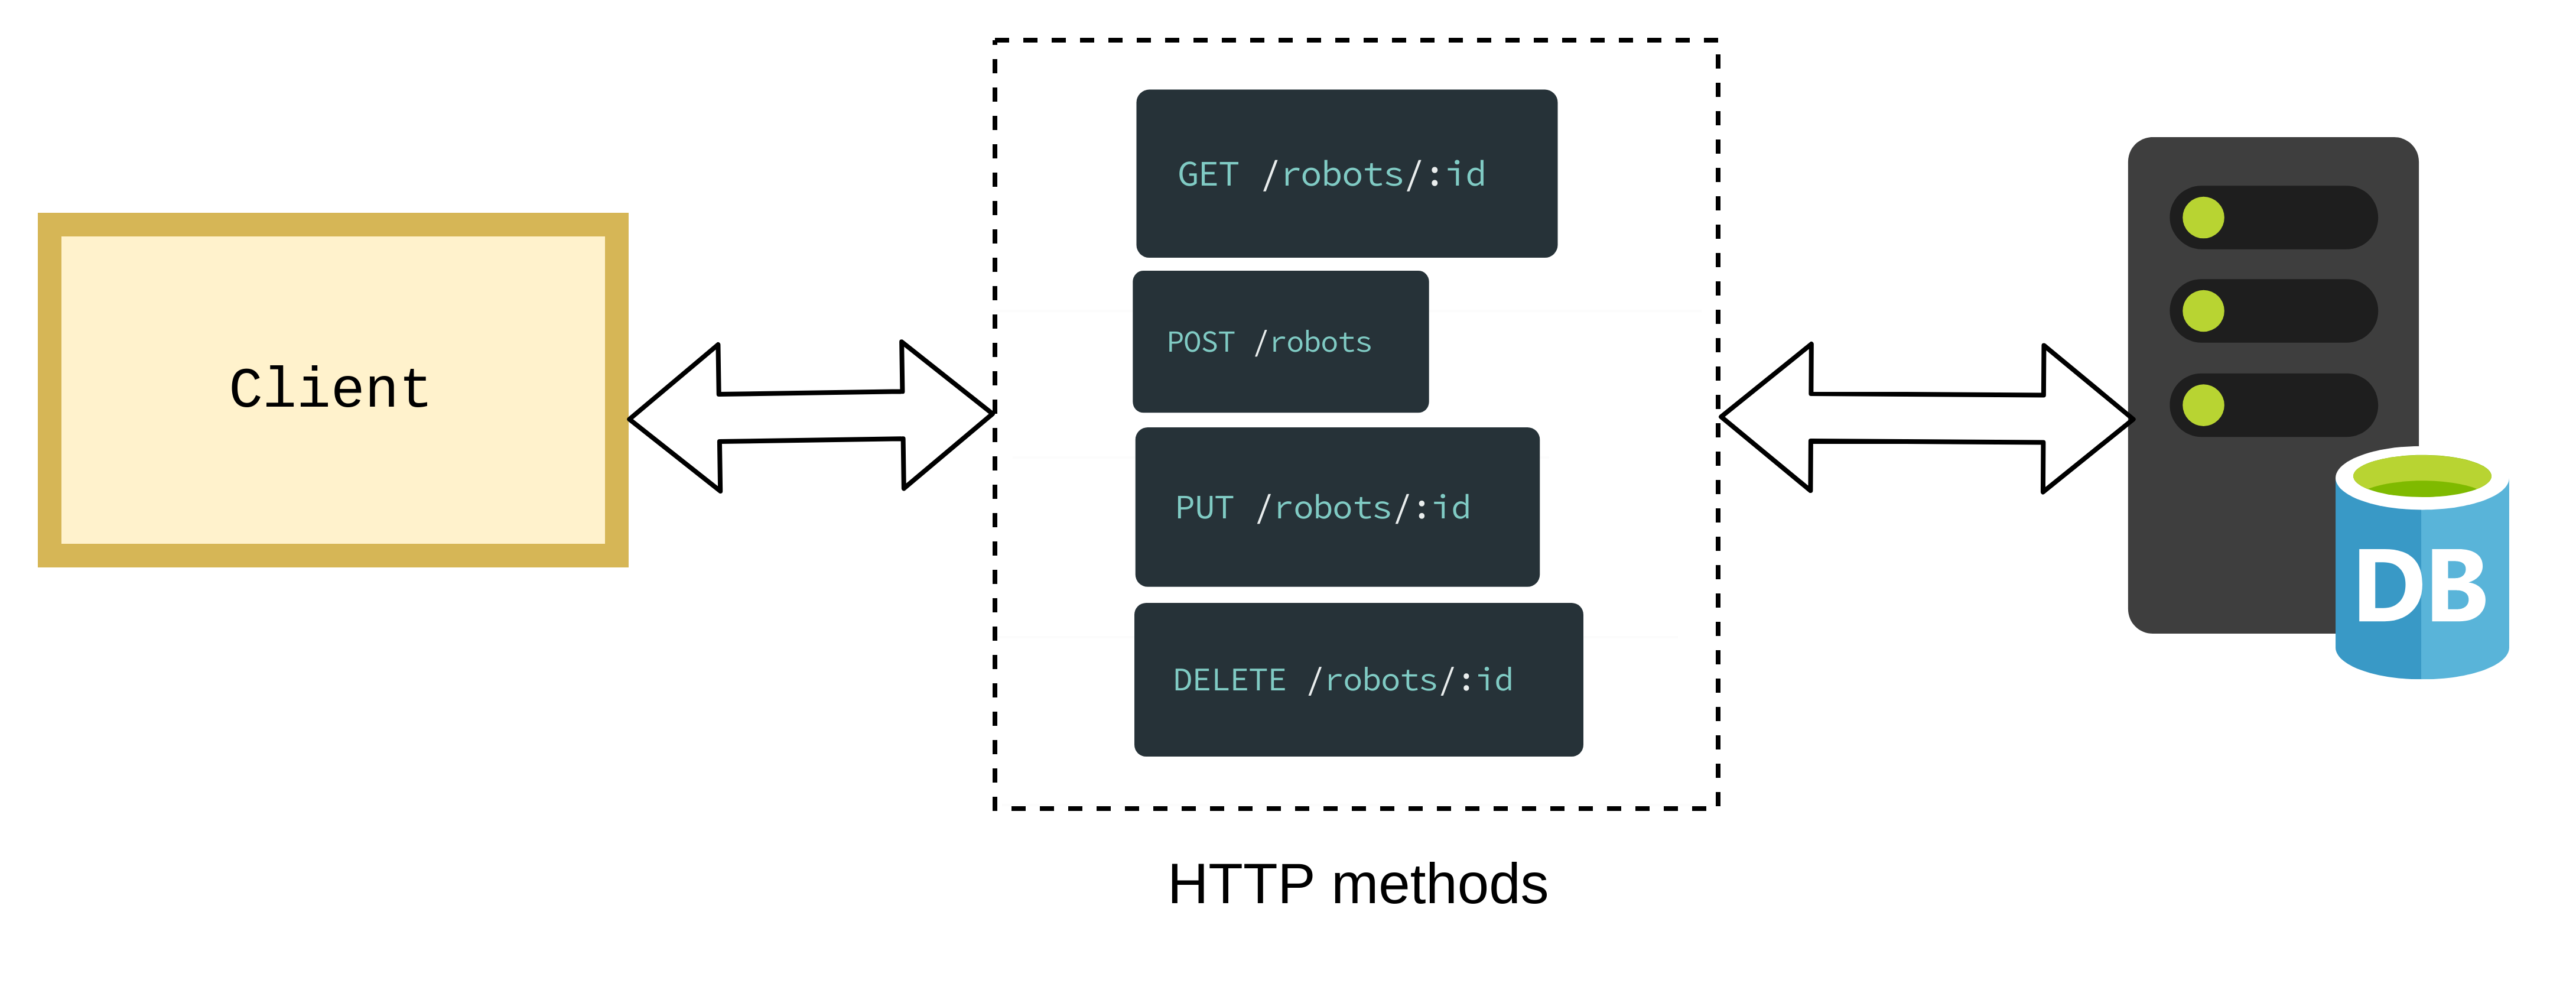
\includegraphics[trim={0 0 0 2cm},clip,scale=0.105]{./images/png/rest_workflow}	
			\caption{Traditional REST API Workflow}	
			\label{fig:rest_workflow}	
		\end{center}
	\end{figure}
	
	\subsubsection{Limitations}
	\begin{itemize}
		\item The client has to make recurring round trips to the server to fetch the required data.
		\item Various endpoints for different resources which make complication between developers and challenging to manage them on server and client side in big projects.
		\item Over Fetching, means there is no way to control the response to include only a subset of fields which bloats the response size and may cause network traffic.
		\item No static type validation on data sent or received.		
	\end{itemize}

	In the later sections, we see how GraphQL and Falcor address the limitations in their approach.
	
	\subsection{GraphQL}
	GraphQL is a Query Language developed by Facebook to fetch the data from the database unlike the traditional way of making REST API requests. Technically, GraphQL replaces the use of REST API calls with a single endpoint on the server. Single endpoint architecture solves various communication difficulties between client and server side team members. 
	
	\subsubsection{Single roundtrip}
	GraphQL helps to fetch all the data we required in a single request. For example, consider a scenario in the below figure where we need to get top 10 robots and sensors attached to it. 
	
	\begin{figure}[!htbp] 
		\begin{center}
			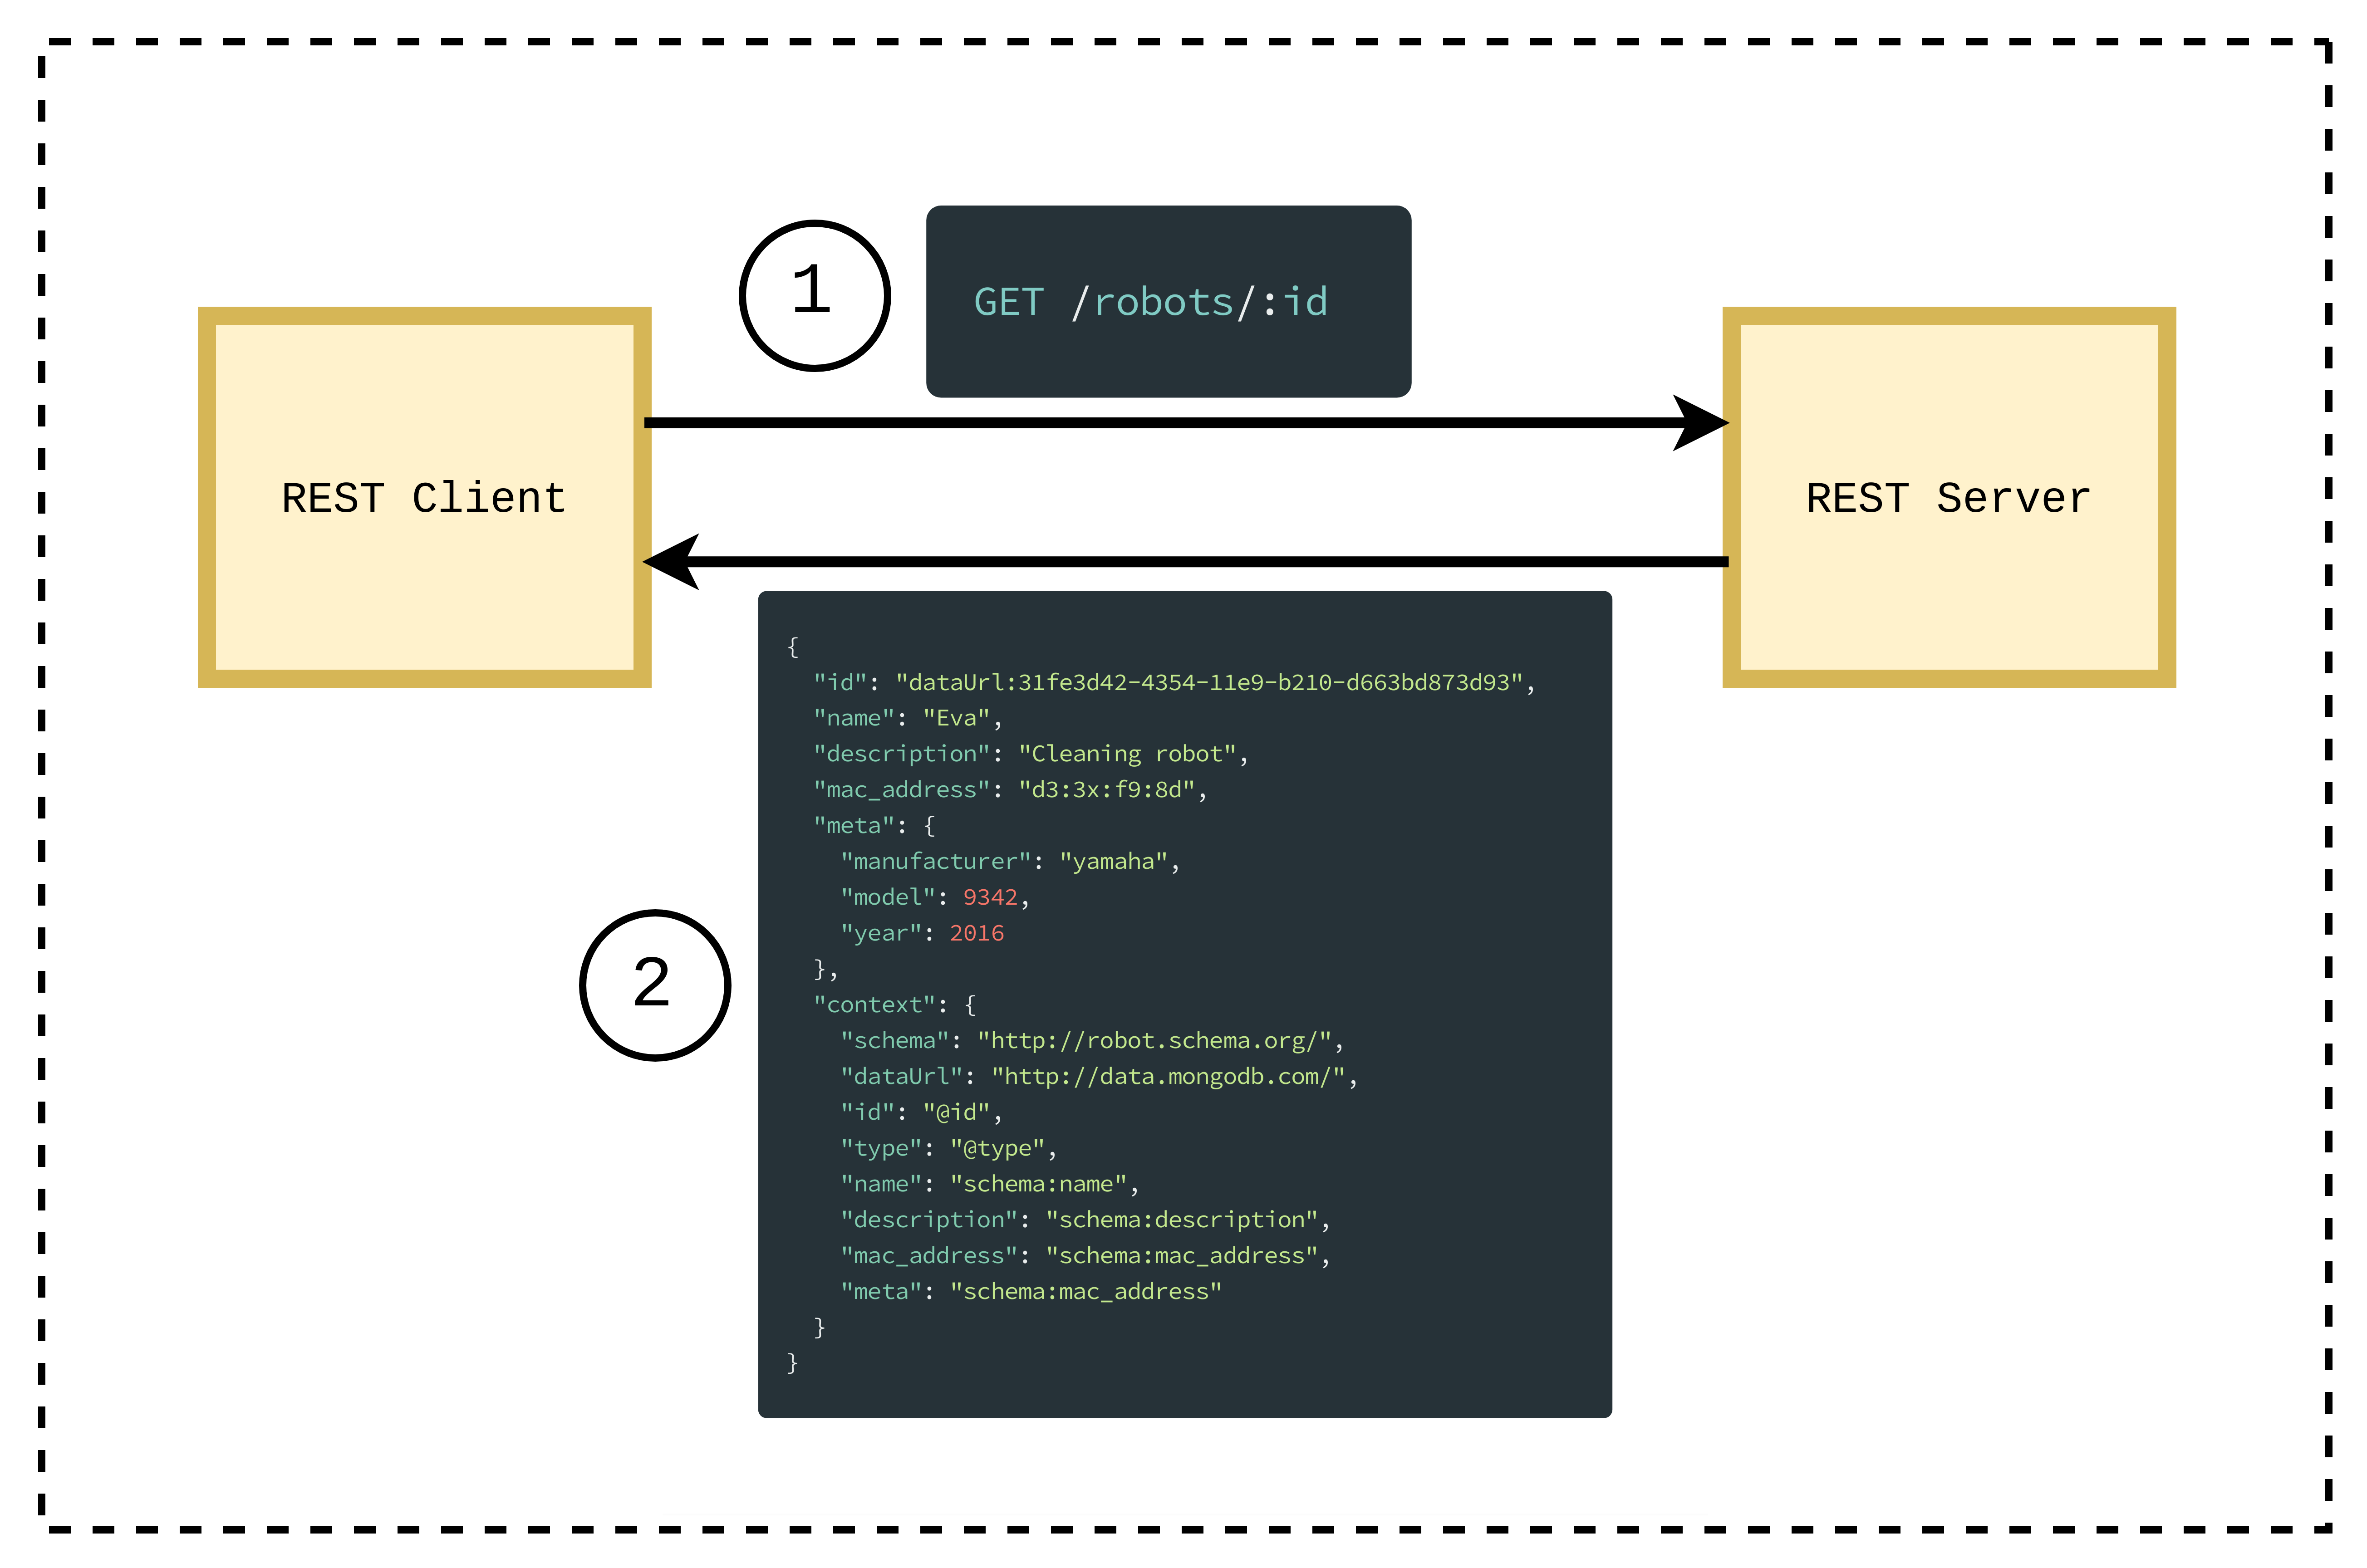
\includegraphics[trim={0 0 0 2cm},clip,scale=0.09]{./images/png/rest_roundtrip_1}	
			\caption{Multiple round trips in REST API (a)}	
			\label{fig:rest_roundtrip_1}	
		\end{center}
	\end{figure}
	
   Figure \ref{fig:rest_roundtrip_1} shows the traditional REST approach, step 1 shows single GET request to fetch a piece of robot information and step 2 shows the JSON response that includes the robot information which is requested. Note that, server spits out all information regardless of what client is going to use in their application. 
   
   In figure \ref{fig:rest_roundtrip_2} step 3 shows the next GET request from the client to fetch all the sensor information belongs to the robot\_id which client received in step 2 response. In step 4, the server responds with all sensor details for the specified robot. 
	
	\begin{figure}[!htbp] 
		\begin{center}
			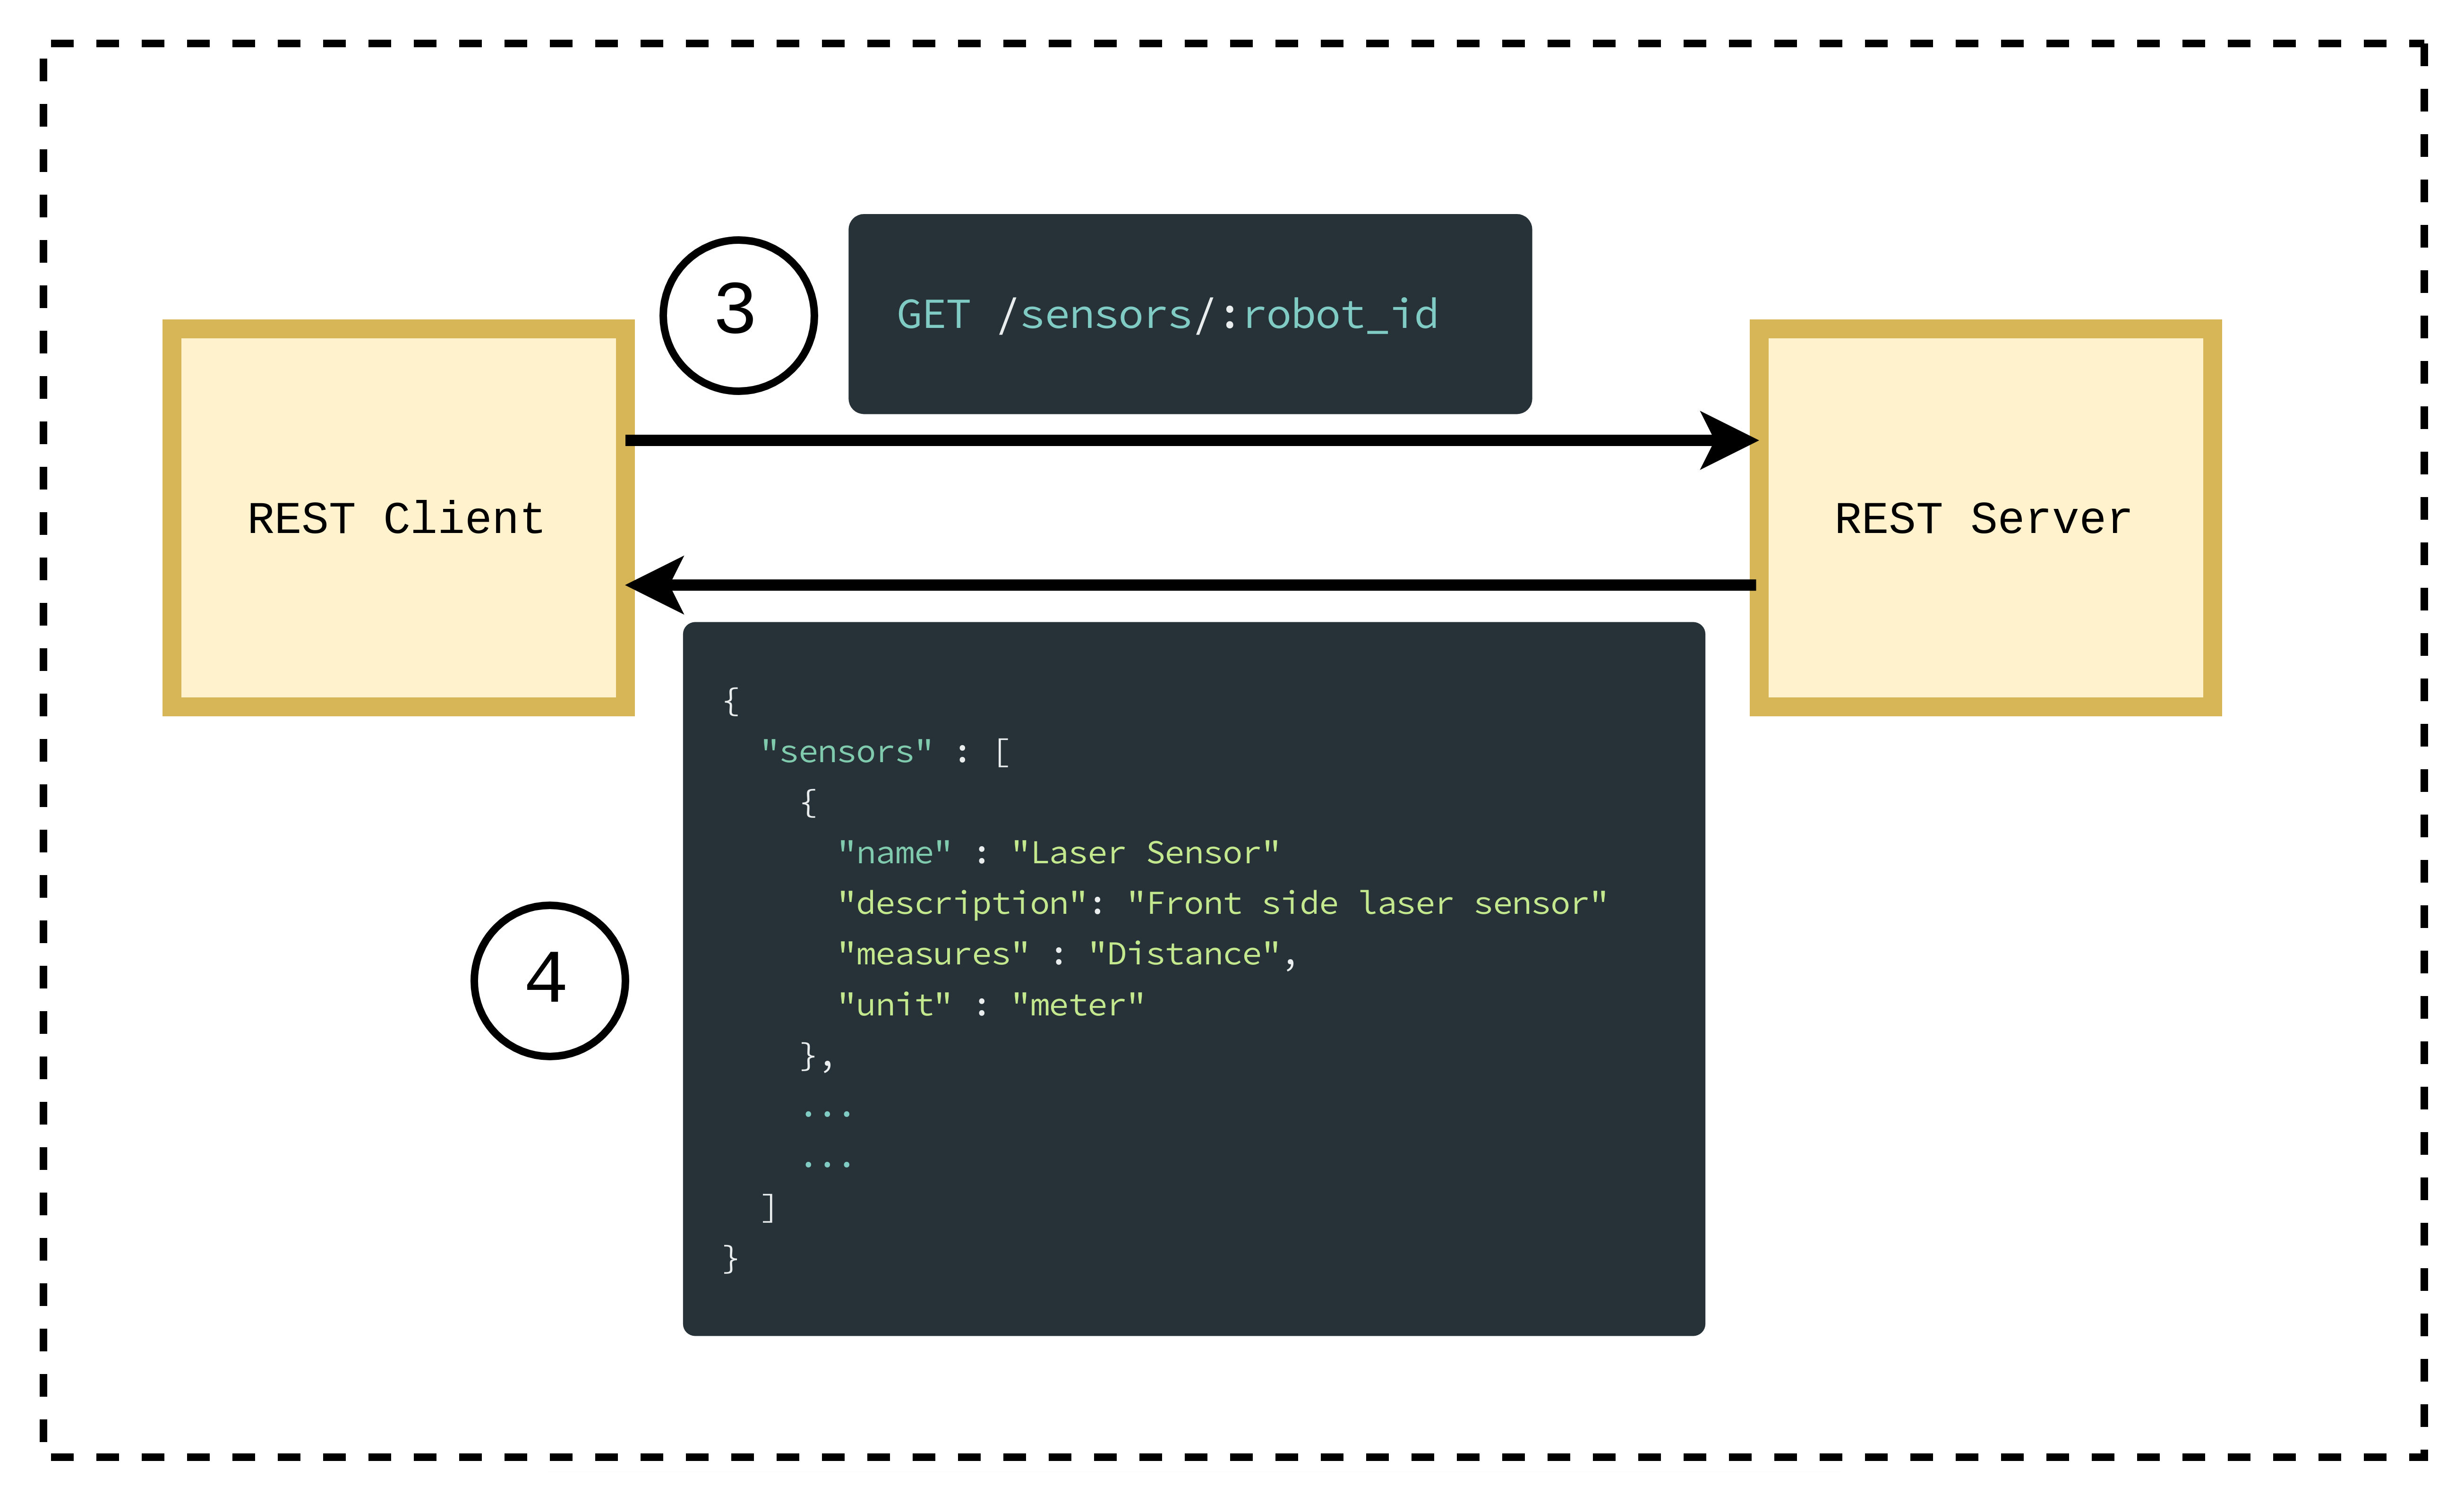
\includegraphics[trim={0 0 0 2cm},clip,scale=0.09]{./images/png/rest_roundtrip_2}	
			\caption{Multiple round trips in REST API (b)}	
			\label{fig:rest_roundtrip_2}	
		\end{center}
	\end{figure}

   To get all 10 robots information, the client has to make a series of individual GET requests to fetch all robots information and later client makes another round of requests to get the sensor data. This consumes too much network resources by making multiple roundtrips.
 
 	On the other hand, figure \ref{fig:graphql_roundtrip} shows that GraphQL client attaches the required fields and their additional related fields in a single request to fetch the complete information in a single roundtrip which reduces the usage of network resources tremendously.  
	
	\begin{figure}[!htbp] 
		\begin{center}
			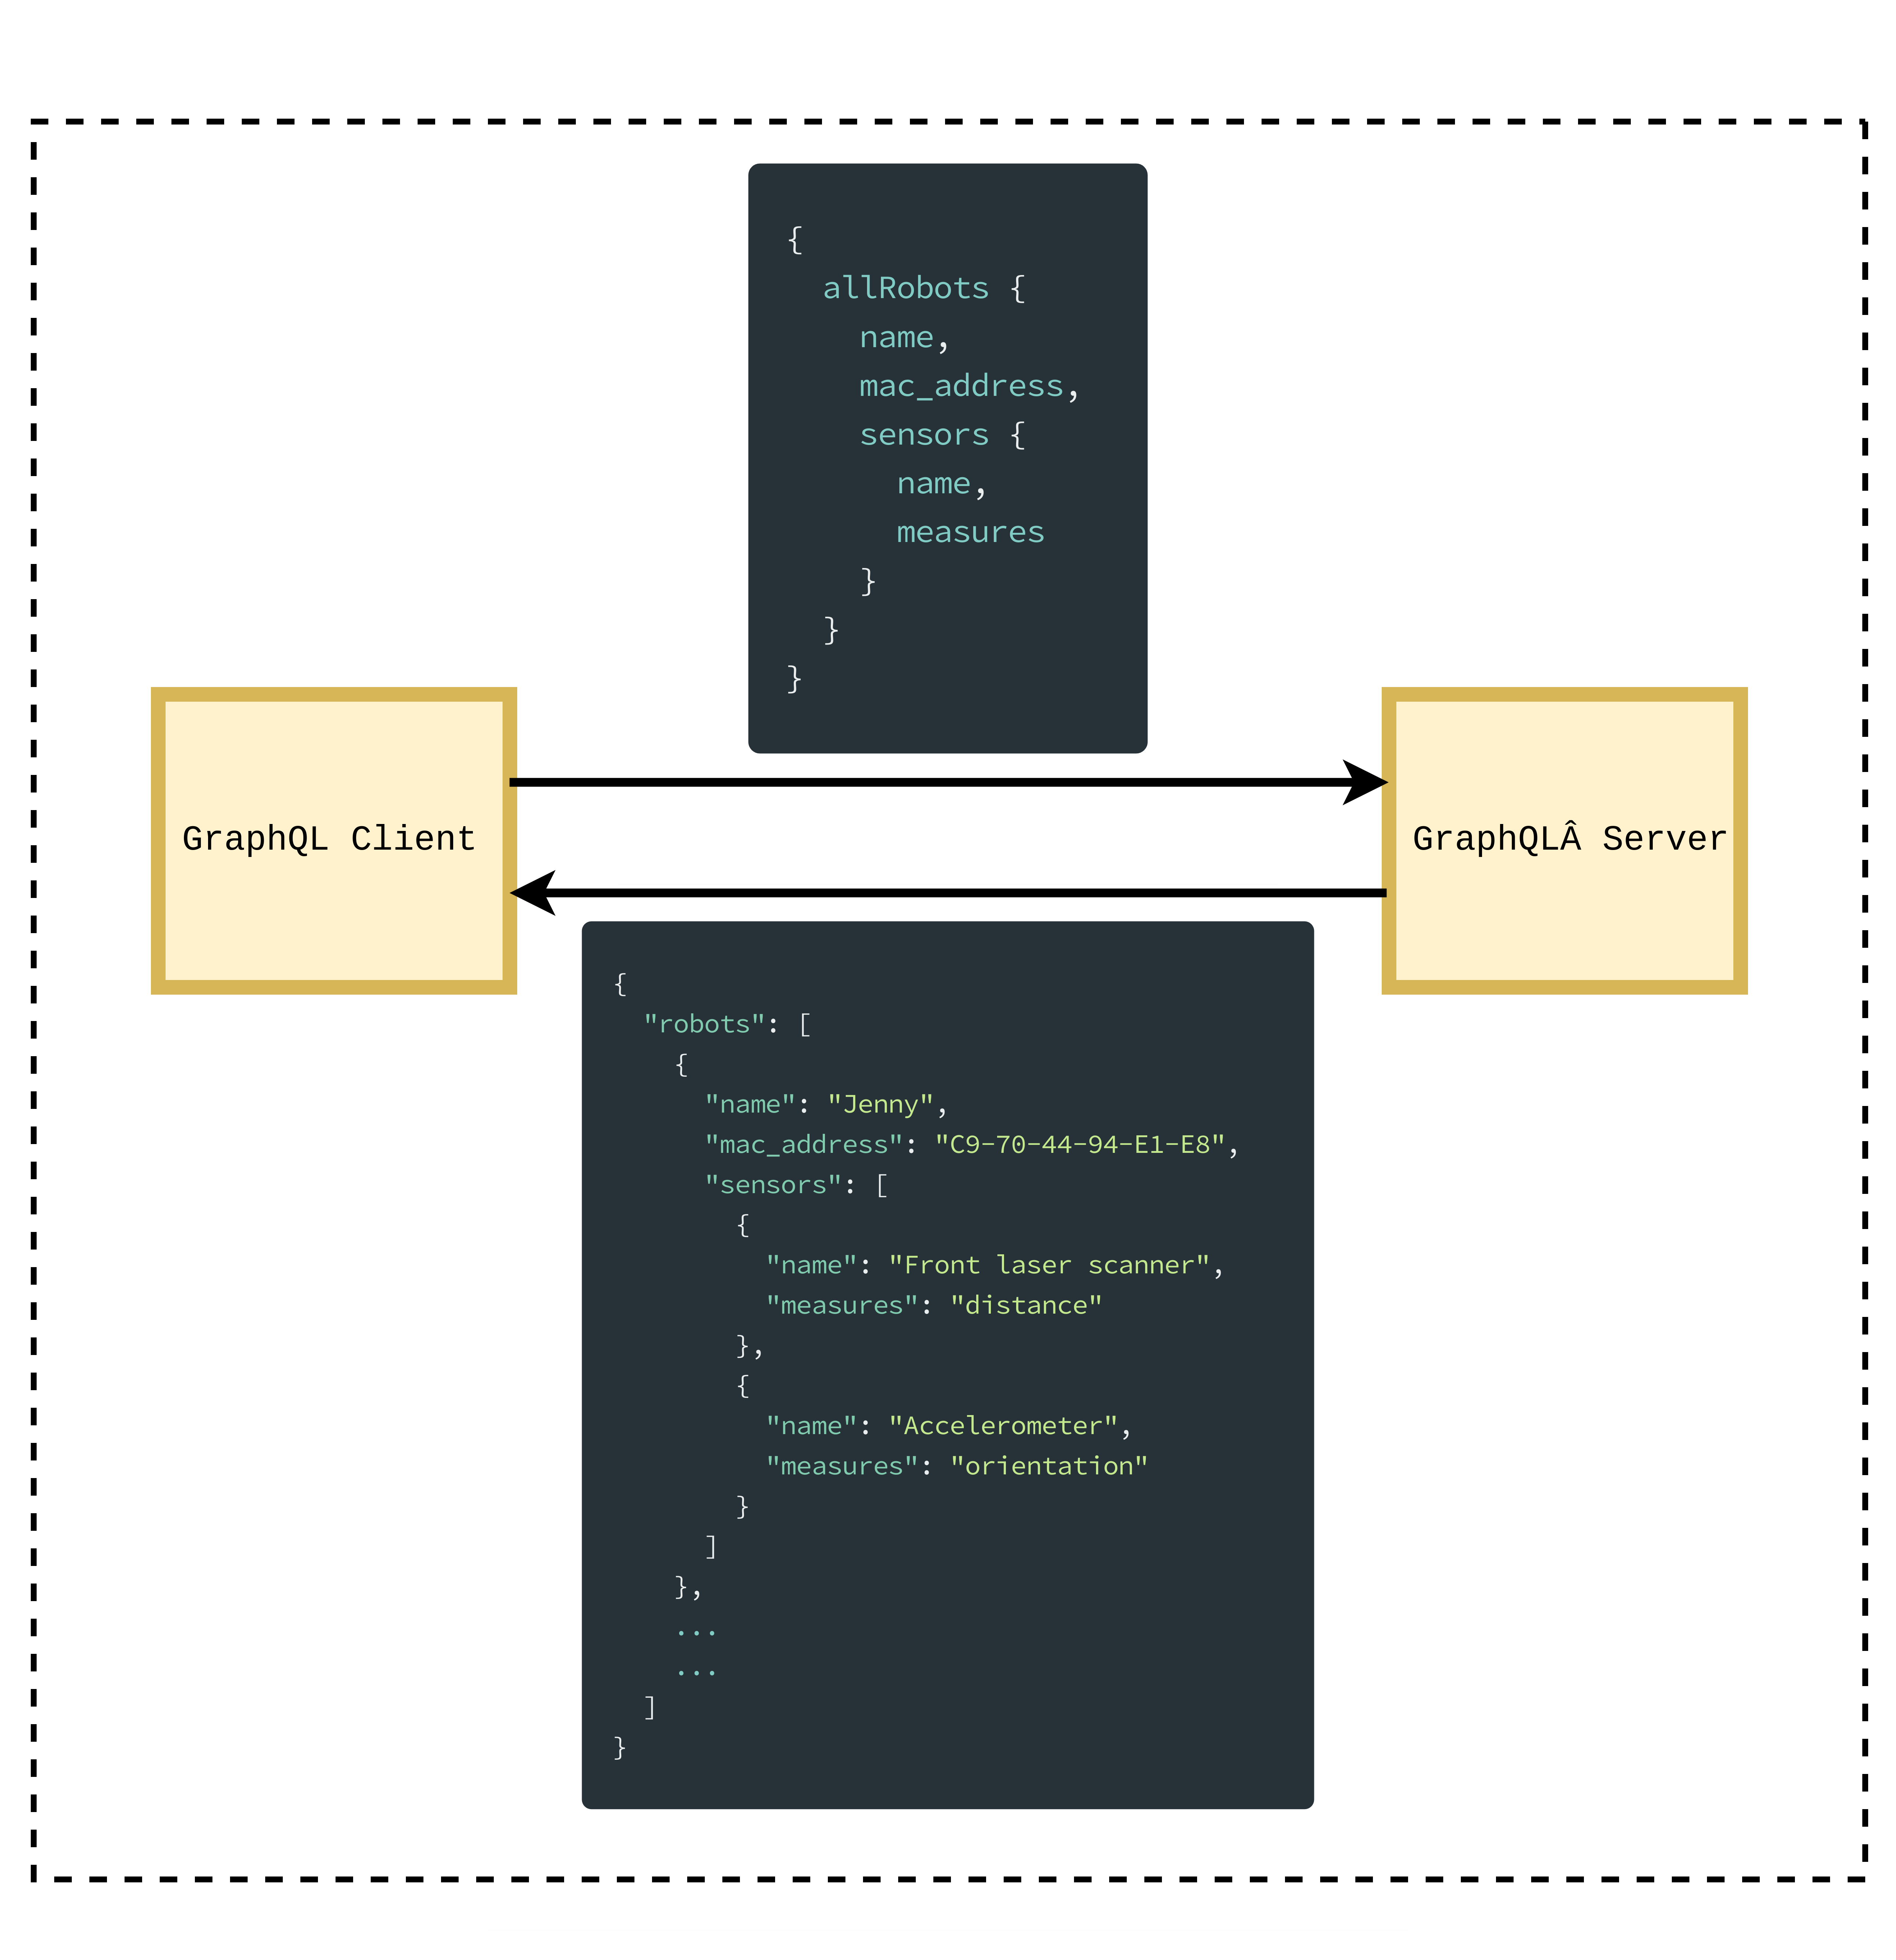
\includegraphics[trim={0 0 0 2cm},clip,scale=0.09]{./images/png/graphql_roundtrip}	
			\caption{Single roundtrip in GraphQL}	
			\label{fig:graphql_roundtrip}	
		\end{center}
	\end{figure}

	\subsubsection{Declarative}
	The client decides the fields that should be available in the query response. GraphQL doesn't give less or more than what the client asks for.  Declarative approach solves the over fetching issue in REST API. Also, we can say that GraphQL follows under fetching approach. 
	
	Let's consider an example to see the variance between these two approaches. Imagine we have a database that contains a list of robot information such as name, description, mac\_address, context, manufacturer information, type, weight, etc. and we would like to query only for name and mac\_address of all the robots. 
	
	\begin{figure}[!htbp] 
		\begin{center}
			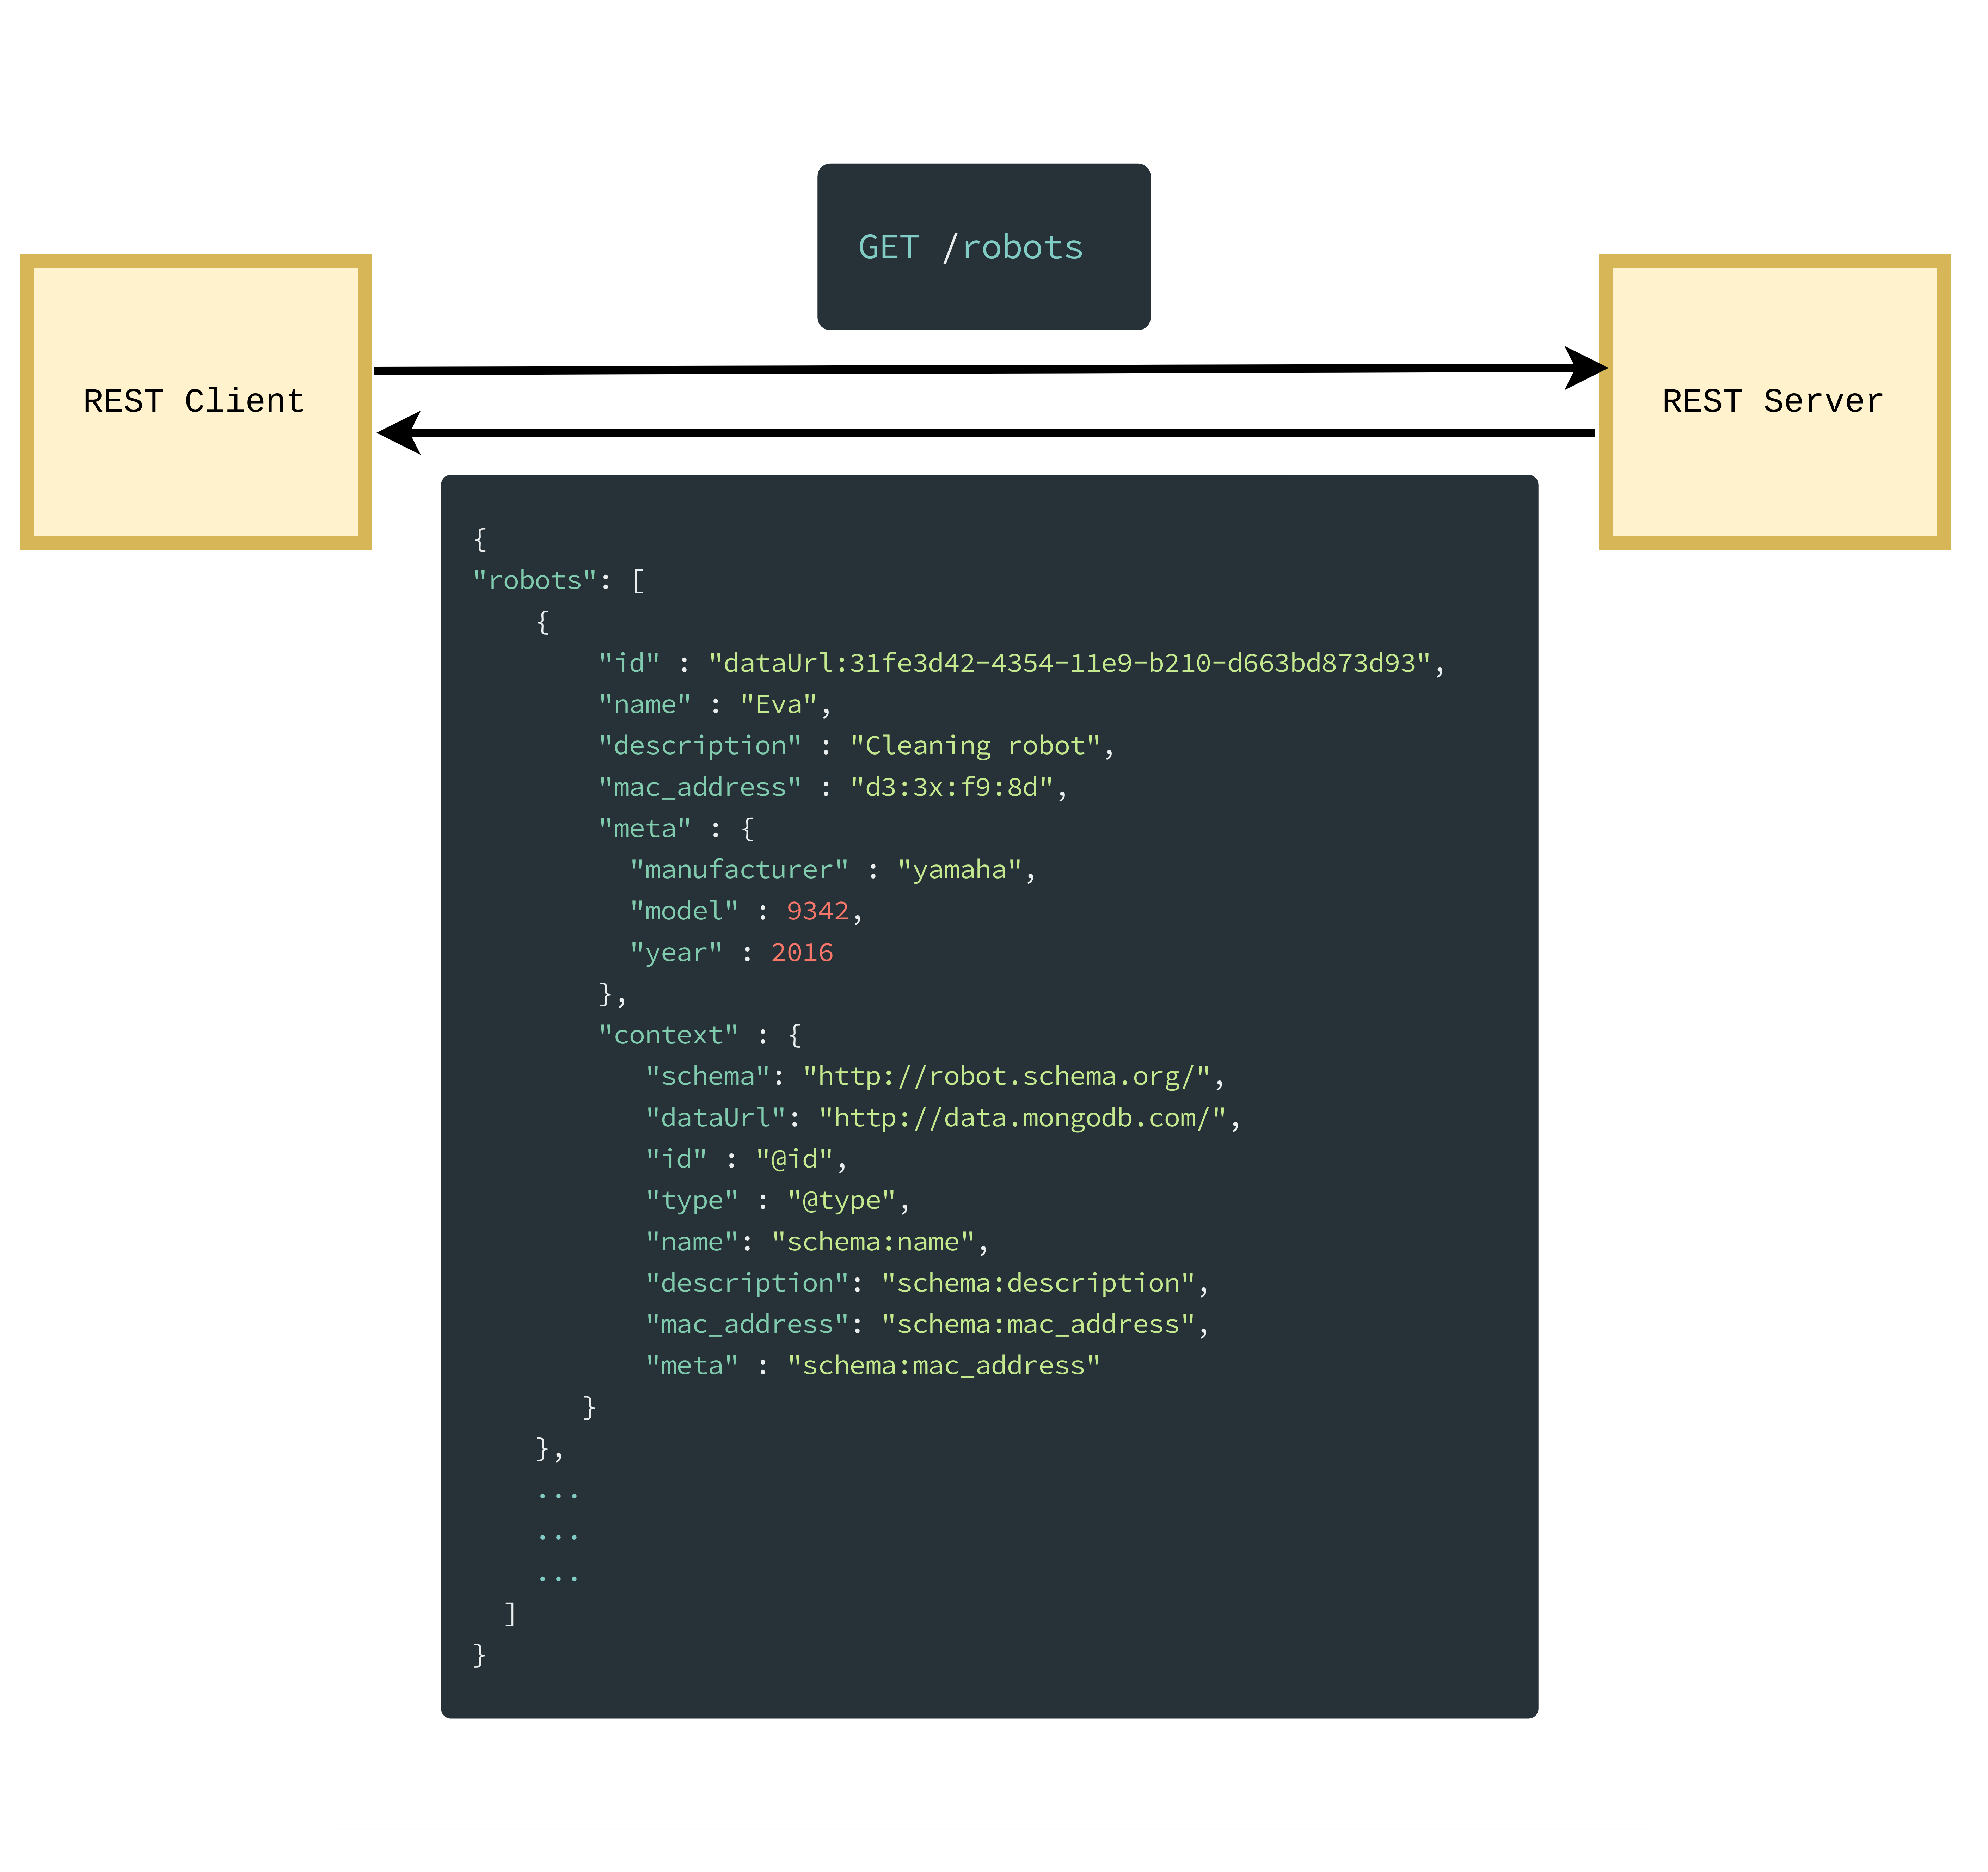
\includegraphics[trim={0 0 0 2cm},clip,scale=0.08]{./images/png/rest_declarative}	
			\caption{Fetching all robot details via REST API includes all the attributes related to each robot.}	
			\label{fig:rest_declarative}	
		\end{center}
	\end{figure}

	In the figure \ref{fig:rest_declarative}, the REST client requests to the server to get all the robots and server returns with a list of robots as a response but each robot object in the response consists of every information belongs to it. Now the client has to handpick the only required fields from the response. 
	Adding \$include=name,mac\_address queries along with the GET request might solve this issue. However, this is overburden in terms of often rewriting code in the server for every change from the client.   
	
	GraphQL solves this over fetching issue with zero configuration in the server side. In the below figure \ref{fig:graphql_declarative}, GraphQL client request for name and mac\_address of all robots exclusively, and GraphQL server automagically responds a list of robots only with name and mac\_address. In the end, it saves time on rewriting code on the server, and most importantly reduces the load on the network layer.
	\newpage
	\begin{figure}[!htbp] 
		\begin{center}
			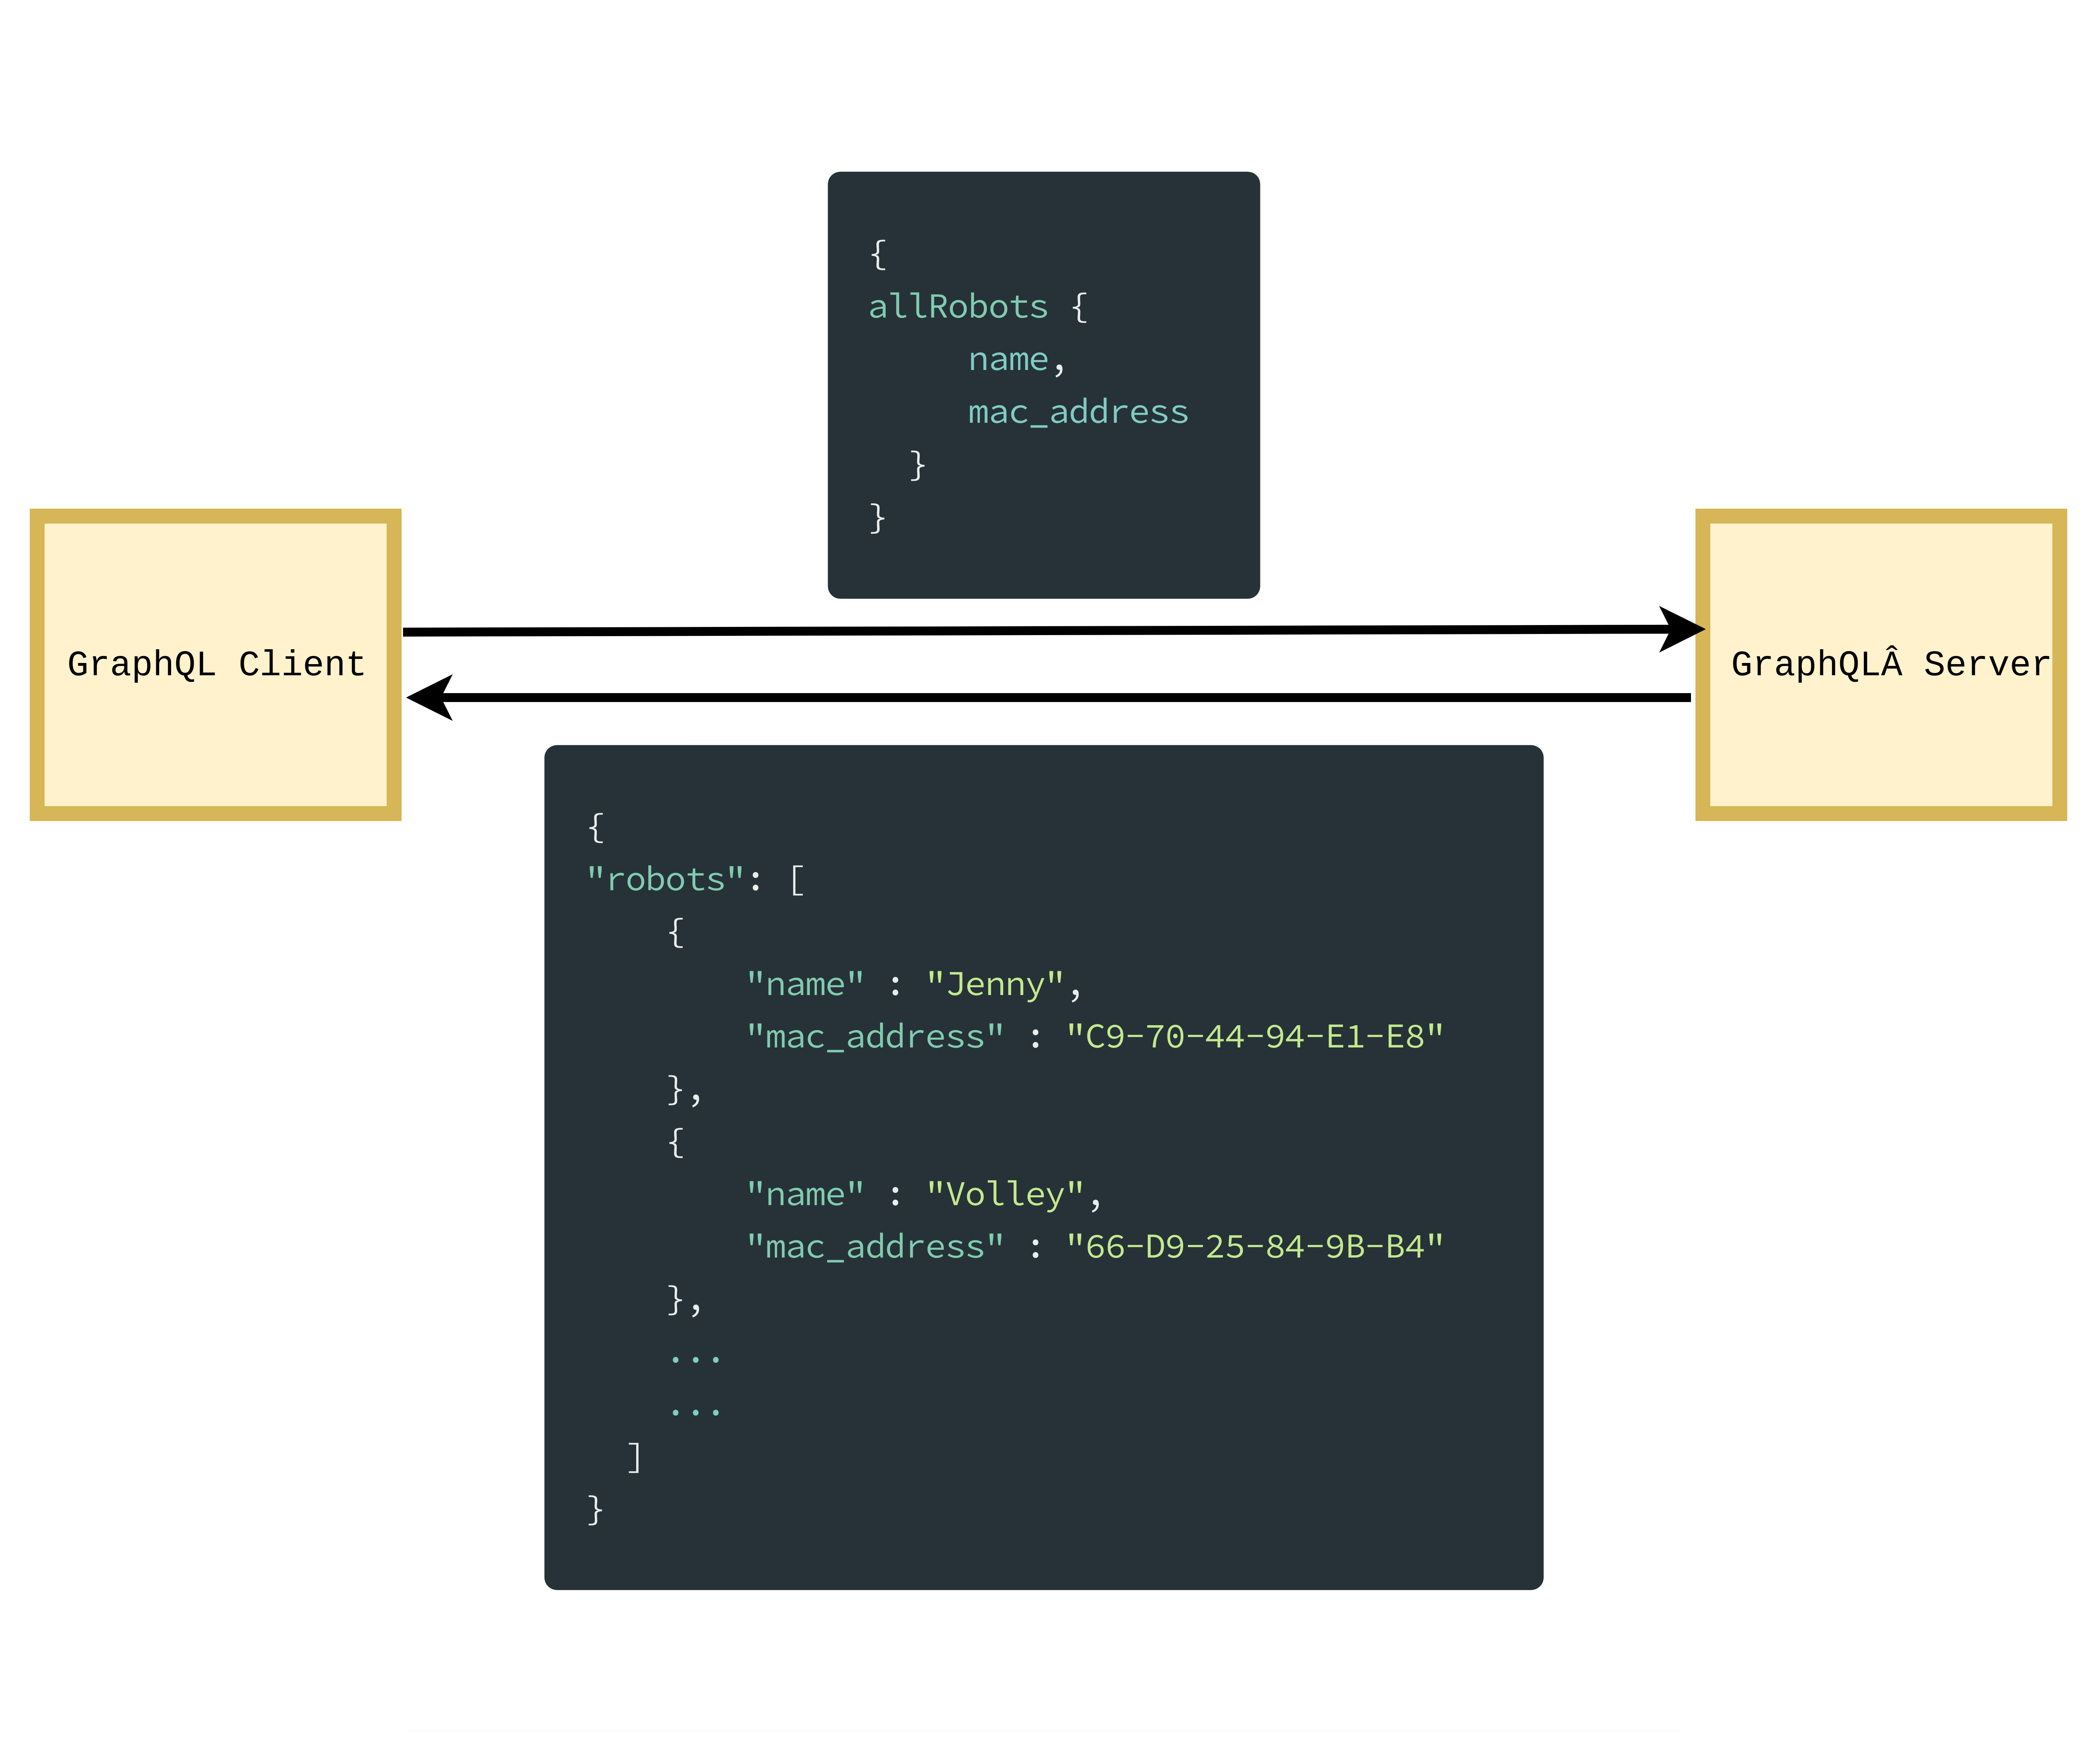
\includegraphics[trim={0 0 0 2cm},clip,scale=0.07]{./images/png/graphql_declarative}	
			\caption{Fetching only required robot details with GraphQL queries}	
			\label{fig:graphql_declarative}	
		\end{center}
	\end{figure}

	\subsubsection{Single endpoint}
	
	GraphQL exposes a single endpoint for all available services from the backend. This overcomes the REST API multiple routes and each exposes a single resource. For example, consider we need to get a list of robots and sensors in two different network calls. In typical REST API architecture, we would have two separate routes as shown below.
	
	"/robots" \& "/sensors"
	
	In GraphQL world, we define only one route, and we send the queries to the server over the single URL.
	
	\subsubsection{Strongly typed validation}
	Strong type system in GraphQL validates the incoming query for data types and prevent prematurely even before sending the queries to the database. Also, it makes sure that the client sends the right data and also the client can expect the data in the same way. 
	
	\subsubsection{Caching}
	Usually, the browser caches the responses for different routes, and if the client makes a similar request, the browser gets the data locally. However, it is not possible directly since GraphQL uses single route endpoint. Without caching, GraphQL would be inefficient, but there are other libraries in the community which handles the caching in the client side. The popular libraries are Apollo and FlacheQL, and they store the requests and responses in the simple local storage in the form of a normalized map \cite{misc02}.
	
	\subsubsection{Multiple data sources}
	GraphQL creates an abstraction layer between clients and the databases used in the backend as shown in the figure \ref{fig:multiple_db_support}. This feature allows the service provides to use any number of data sources and GraphQL fetches the relevant data from all data sources and returns the required fields to the client side. 
	
	This is one of the primary reason why we considered GraphQL as a base to our mediator system. Because it is always not sure how the robots store the sensor data and which database is used. In a typical scenario, multi robots might use various databases to store similar sensor entities.

	\begin{figure}[!htbp] 
		\begin{center}
			\includegraphics[trim={0 0 0 2cm},clip,scale=0.07]{./images/png/multiple_db_support}	
			\caption{ Connecting multiple data sources with GraphQL}	
			\label{fig:multiple_db_support}	
		\end{center}
	\end{figure}

	\subsection{Falcor}
	Falcor is a framework similar to GraphQL developed by Netflix for their internal use, and later they made it available as open source. Unlike GraphQL, Falcor doesn't emphasize users to provide a schema. Instead, Falcor generates a schema from the given data as a single Virtual JSON object \cite{misc03}. It uses "One Model Everywhere" \cite{misc03} policy to model all the backend data into a single JSON file.
	
	\begin{figure}[!htbp] 
		\begin{center}
			\includegraphics[trim={0 0 0 2cm},clip,scale=0.09]{./images/png/one_model_everywhere}	
			\caption{ Falcor One Model Everywhere design \cite{misc03} }	
			\label{fig:one_model_everywhere}	
		\end{center}
	\end{figure}
	Falcor and GraphQL share many similarities like data demand driven architecture, single endpoint, single roundtrip, and under fetching.
	
	However, what makes Falcor differ from GraphQL and why limited people are using the Falcor framework compared to GraphQL. The major reasons are,
	\begin{itemize}
		\item Falcor is not a query language like GraphQL. Alternately, Falcor uses a javascript style of accessing attributes from the objects to select the necessary fields in the response.
		\item It works based on a single colossal JSON model.
		\item Falcor doesn't follow a strong type validation out of the box, and the users may achieve this functionality manually with one of the popular type systems like JSON schema or typescript.
		\item By default, GraphQL provides schema introspection which allows various tools to utilize the representation of schema beforehand. Though, Falcor says, "if you know your data, you know your API" \cite{misc04} which is not true always since more often we don't know what fields and their names available in our data.
		\item GraphQL have a wide range of server implementation in C\# / .NET, Clojure, Elixir, Erlang, Go, Groovy, Java, JavaScript, PHP, Python, Scala, Ruby \cite{misc05}. Unfortunately, Falcor has their implementations in JavaScript, Java and C\# / .NET. This hardly gives options for the developers to choose Falcor.
		\item It is possible in GraphQL to pass arguments to queries which allow the user to do advanced operations in the backend. However currently, Falcor doesn't support this feature.
	\end{itemize}

	Falcor also has few advantages over GraphQL. 
	\begin{itemize}
		\item Easy learning curve.
		\item Simple to adapt with small range projects.
		\item Caching and query merging.
		\item Batching and Deduplication \cite{misc06}.
	\end{itemize}

	\subsection{Conclusion} \label{sec:graphql_falcor_conclusion}
	At the end of this research work, we develop a mediator component to interact with diverse databases running in multi-robot systems. For that, we need to decide to choose between GraphQL and Falcor as a base for the mediator component since they have the capabilities to fetch data from various data sources and return a single response over a single endpoint. However, for choosing one we have made a detailed comparison in the above sections based on their abilities and features. Most of the times, GraphQL supersede Falcor in case of flexibility, scalability, introspection, type validation, and more language support. So we conclude to use GraphQL as a base for our mediator component.
\end{document}
